\vspace{-0.2cm}
\section{When Can Offline RL Initializations Enable Fast Online Fine-Tuning?}
\label{sec:empirical}
\vspace{-0.2cm}

A starting point for offline pre-training and online fine-tuning is to simply initialize the value function with one that is produced by an existing offline RL method and then perform fine-tuning. However, we empirically find that initializations learned by many offline RL algorithms can perform poorly during fine-tuning. We will study the reasons for this poor performance for the subset of conservative methods to motivate and develop our approach for online fine-tuning, calibrated Q-learning. 

\vspace{-0.1cm}
\subsection{Empirical Analysis}
\label{sec:empirical_analysis}
\vspace{-0.2cm}

\begin{wrapfigure}{r}{0.38\columnwidth}
\vspace{-1.0cm}
\begin{center}
{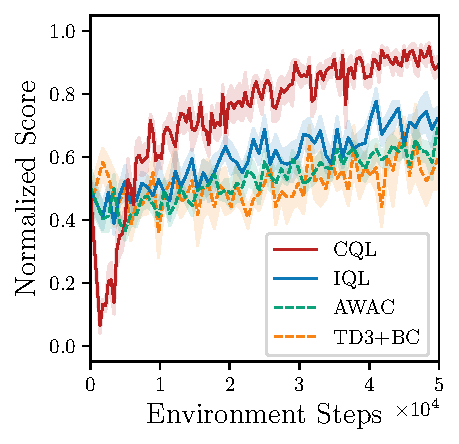
\includegraphics[width=0.78\linewidth]{chapters/cal_ql/figs-sample/sec41-final-utd5.pdf}}
\vspace{-0.3cm}
\caption{\label{fig:cql_iql_finetune}\footnotesize{\textbf{Multiple prior offline RL algorithms suffer from difficulties} during fine-tuning including poor asymptotic performance and initial unlearning.}}
\vspace{-0.7cm}
\end{center}
\end{wrapfigure}
Offline RL followed by online fine-tuning typically poses non-trivial challenges for a variety of methods. While analysis in prior work~\citep{nair2020accelerating} notes challenges for a subset of offline RL methods, in Figure~\ref{fig:cql_iql_finetune}, we evaluate the fine-tuning performance of a variety of prior offline RL methods (CQL~\citep{kumar2020conservative}, IQL~\citep{kostrikov2021offlineb}, TD3+BC~\citep{fujimoto2021minimalist}, AWAC~\citep{nair2020accelerating}) on a particular diagnostic instance of a visual pick-and-place task with a distractor object and sparse binary rewards~\citep{singh2020cog}, and find that all methods struggle to attain the best possible performance, quickly. More details about this task are in Appendix~\ref{appendix:env_details}. 

% The analysis by \citet{nair2020accelerating} highlights the limitations of explicit policy constraint methods for fine-tuning. Therefore, in this section, we study a representative \emph{implicit} policy constraint method, implicit Q-learning (IQL)~\cite{kostrikov2021offlineb} that attains good performance on benchmark tasks, and a conservative method, CQL~\cite{kumar2020conservative}.
%%SL.5.7: I really think we should just remove the IQL discussion here. We don't actually "study" IQL in any meaningful way here, and the reference to Nair et al. is pretty tortured too. We could just say we'll use CQL as our starting point, though the issues we observe have also been noted with other RL methods (and we can reference Nair for that, since the AWAC paper also observes the "dip").
%%SZ.5.9: agree
% We study the task of fine-tuning a robot policy on a visual pick-and-place task with a distractor object and sparse binary rewards, from prior work~\cite{singh2020cog}. 
% More details about the offline dataset are in Appendix~\ref{appendix:env_details}.  

% We present the learning curves for both methods in online fine-tuning in Figure~\ref{fig:cql_iql_finetune}. 
While the offline Q-function initialization obtained from all methods attains a similar (normalized) return of around 0.5, they suffer from difficulties during fine-tuning: TD3+BC, IQL, AWAC attain slow asymptotic performance and CQL unlearns the offline initialization, followed by spending a large amount of online interaction to recover the offline performance again, before any further improvement. This initial unlearning appears in multiple tasks as we show in Appendix~\ref{app:cql_dip_zoom_in}. In this work, we focus on developing effective fine-tuning strategies on top of conservative value estimation methods like CQL. To do so, we next aim to understand the potential reason behind the initial unlearning in CQL.  

\begin{wrapfigure}{r}{0.6\linewidth}
\vspace{-0.5cm}
\begin{center}
\centerline{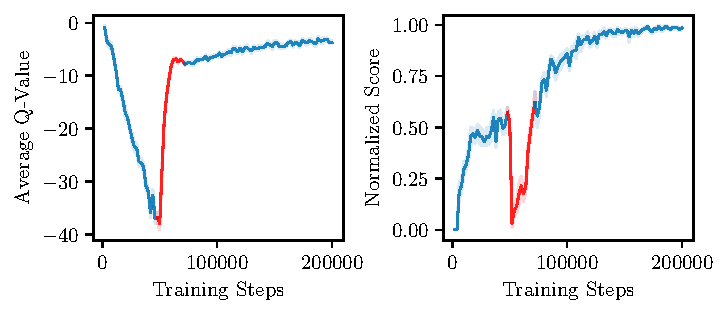
\includegraphics[width=0.99\linewidth]{chapters/cal_ql/figs-sample/CQL-q-values.pdf}}
\vspace{-0.25cm}
\caption{\label{fig:cql_q_value} \footnotesize{\textbf{The evolution of the average Q-value and the success rate of CQL over the course of offline pre-training and online fine-tuning.} Fine-tuning begins at 50K steps. The red-colored part denotes the period of performance recovery which also coincides with the period of Q-value adjustment.}}
\end{center}
\vspace{-0.7cm}
\end{wrapfigure}
\textbf{Why does CQL unlearn initially?} To understand why CQL unlearns initially, we inspect the learned Q-values averaged over the dataset in Figure~\ref{fig:cql_q_value}. Observe that the Q-values learned by CQL in the offline phase are \emph{much} smaller than their ground-truth value (as expected), but these Q-values drastically jump and adjust in scale when fine-tuning begins. In fact, we observe that performance recovery (red segment in Figure~\ref{fig:cql_q_value}) {\em coincides} with a period where the range of Q-values changes to match the true range. This is as expected: as a conservative Q-function experiences new online data, actions much worse than the offline policy on the rollout states appear to attain higher rewards compared to the highly underestimated offline Q-function, which in turn deceives the policy optimizer into unlearning the initial policy. We illustrate this idea visually in Figure~\ref{fig:calql_idea}. Once the Q-function has adjusted and the range of Q-values closely matches the true range, then fine-tuning can proceed normally, after the dip. 


\textbf{To summarize,} our empirical analysis indicates that methods existing fine-tuning methods suffer from difficulties such as initial unlearning or poor asymptotic performance. In particular, we observed that conservative methods can attain good asymptotic performance, but ``waste'' samples to correct the learned Q-function. Thus, in this paper, we attempt to develop a good fine-tuning method that builds on top of an existing conservative offline RL method, CQL, but aims to ``calibrate'' the Q-function so that the initial dip in performance can be avoided. 

\vspace{-0.1cm}
\subsection{Conditions on the Offline Initialization that Enable Fast Fine-Tuning}
\vspace{-0.18cm}
Our observations from the preceding discussion motivate two conclusions in regard to the offline Q-initialization for fast fine-tuning: \textbf{(a)} methods that learn \textbf{conservative} Q-functions can attain good asymptotic performance, and \textbf{(b)} if the learned Q-values closely match the range of ground-truth Q-values on the task, then online fine-tuning does not need to devote samples to unlearn and then recover the offline initialization. One approach to formalize this intuition of Q-values lying on a similar scale as the ground-truth Q-function is via the requirement that the conservative Q-values learned by the conservative value estimation method must be lower-bounded by the ground-truth Q-value of a sub-optimal reference policy. This will prevent conservatism from learning overly small Q-values. We will refer to this property as ``calibration'' with respect to the reference policy.
\begin{tcolorbox}[colback=blue!6!white,colframe=black,boxsep=0pt,top=-3pt,bottom=2pt]
\vspace{5mm}
\begin{definition}[Calibration]
\label{cond:calibration}
An estimated Q-function ${Q}_\theta^\pi$ for a given policy $\pi$ is said to be calibrated with respect to a reference policy $\mu$ if:
\begin{align} 
    \mathbb{E}_{\mathbf{a} \sim \pi}\left[Q_\theta^\pi(\bs, \mathbf{a})\right] \geq \mathbb{E}_{\mathbf{a} \sim \mu}\left[Q^\mu(\bs, \mathbf{a})\right] := V^\mu(s), \forall s \in \mc \mathcal{D}.
\end{align}
\end{definition}
\end{tcolorbox}

If the learned Q-function ${Q}^\pi_\theta$ is calibrated with respect to a policy $\mu$ that is worse than $\pi$, it would prevent unlearning during fine-tuning that we observed in the case of CQL.
This is because the policy optimizer would not unlearn $\pi$ in favor of a policy that is worse than the reference policy $\mu$ upon observing new online data as the expected value of $\pi$ is constrained to be larger than $V^\mu$: $\mathbb{E}_{\mathbf{a} \sim \pi}\left[{Q}^\pi_\theta(\bs, \mathbf{a})\right] \geq V^\mu(\bs)$.
Our practical approach \methodname\ will enforce calibration with respect to a policy $\mu$ whose ground-truth value, $V^\mu(\bs)$, can be estimated reliably without bootstrapping error (e.g., the behavior policy induced by the dataset). This is the key idea behind our method (as we will discuss next) and is visually illustrated in Figure~\ref{fig:calql_idea}.

\vspace{-0.2cm}